\section{Parallel Programming Models and pthreads}

\subsection{How to create parallel algorithms and programs}

Although \emph{parallel algorithms} and \emph{parallel programs} are in the same father set, the parallel computing topic, these two arguments are a little different.

\begin{definitionbox}[: Parallel Algorithms]
    A \definitionWithSpecificIndex{parallel algorithm}{Parallel Algorithm}{}, as opposed to a traditional serial algorithm, is an \textbf{algorithm which can do multiple operations in a given time}.
\end{definitionbox}

\begin{definitionbox}[: Parallel Programs]
    A \definitionWithSpecificIndex{parallel program}{Parallel Program}{} is a \textbf{program that uses multiple CPU cores}, with \textbf{each core performing a task independently}.
\end{definitionbox}

\noindent
However, designing \emph{parallel algorithms} is not an easy task because there is no heuristic for designing \emph{parallel algorithms}. There are some rules that help in the design. The same reasoning applies to \emph{parallel programs}, because they depend on the chosen language and architecture.

\highspace
Furthermore, there is no single correct solution, but several possible parallel solutions. A \textbf{good first approach is to start with machine-independent issues} (concurrency) and \textbf{delay target-specific issues as much as possible}.

\begin{table}[!htp]
    \centering
    \begin{tabular}{@{} p{16em} p{16em} @{}}
        \toprule
        Design a parallel algorithm & Design a parallel program \\
        \midrule
        Understand the problem to be solved & Analyze the target architecture(s) \\
        \cmidrule{1-2}
        Analyze data dependencies & Choose the best parallel programming model and language \\
        \cmidrule{1-2}
        Partition the solution & Analyze the communications (cost, latency, bandwidth, visibility, synchronization, etc.) \\
        \bottomrule
    \end{tabular}
    \caption{Design parallel algorithms and parallel programs.}
\end{table}

\noindent
The \definition{PCAM (Partitioning, Communication, Agglomeration, Mapping)} methodology described by \href{https://www.mcs.anl.gov/~itf/dbpp/text/node15.html}{Argonne National Laboratory} is intended to promote an exploratory \textbf{approach to design in which machine independent issues}, such as \emph{concurrency}, are \textbf{considered early} and \textbf{machine specific aspects of design are deferred until late in the design process}. In other words, we immediately consider the machine-independent issues (e.g., concurrency) at the beginning of the design approach, and all machine-specific aspects are postponed to an advanced stage of the design process.

\newpage
\noindent
This methodology structures the design process into \textbf{four distinct stages}: 
\begin{enumerate}
    \item \textbf{\underline{Partitioning}}. The \textbf{computation} that is to be performed and the \textbf{data} operated on by this computation are \textbf{decomposed into small tasks}. Practical issues such as the number of processors in the target computer are ignored, and attention is focused on recognizing opportunities for parallel execution.

    \item \textbf{\underline{Communication}}. The communication required to \textbf{coordinate task execution} is determined, and appropriate \textbf{communication structures and algorithms are defined}.

    \item \textbf{\underline{Agglomeration}}. The task and \textbf{communication structures} defined in the first two stages of a design are \textbf{evaluated with respect to performance requirements and implementation costs}. If necessary, tasks are combined into larger tasks to improve performance or to reduce development costs.     

    \item \textbf{\underline{Mapping}}. \textbf{Each task is assigned to a processor} in a manner that attempts to satisfy the competing goals of \textbf{maximizing processor utilization} and \textbf{minimizing communication costs}. Mapping can be specified statically or determined at runtime by load-balancing algorithms.
\end{enumerate}
In the \textbf{first two stages}, we focus on \example{concurrency} and \example{scalability} and seek to \textbf{discover algorithms with these qualities}. In the \textbf{third and fourth stages}, attention shifts to \example{locality} and \example{other performance-related issues}.
\begin{figure}[!htp]
    \centering
    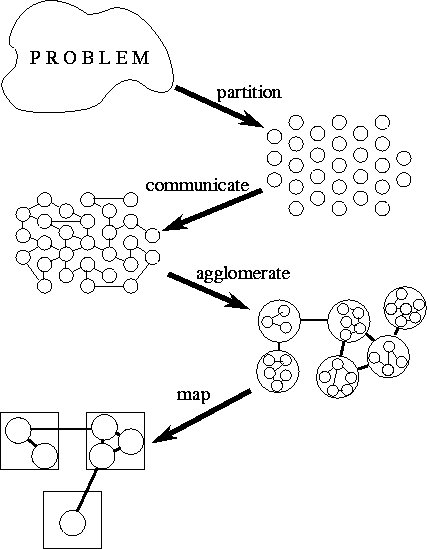
\includegraphics[width=.5\textwidth]{img/pcam-1.png}
    \caption{PCAM design methodology for parallel programs. Starting with a problem specification, develop a partition, determine communication requirements, agglomerate tasks, and finally map tasks to processors.}
\end{figure}